\documentclass[a4paper]{article}

\usepackage[english]{babel}
\usepackage[left=2.5cm,right=2.5cm,top=1cm,bottom=1.5cm]{geometry}
\usepackage[utf8]{inputenc}
\usepackage{amsmath}
\usepackage{amsthm}
\usepackage{amsfonts}
\usepackage{amssymb}
\usepackage{graphicx}
\usepackage{cite}
\usepackage{graphicx}
\usepackage{caption}
\usepackage{subcaption}
\usepackage[colorinlistoftodos]{todonotes}

\usepackage{epsfig}
\usepackage{float}
\usepackage[justification=centering]{caption}

\title{Simulated annealing algorithm for graph coloring}

\author{Xavier Fontaine, Thomas Grivaz, Antoine Mougeot}

\date{\today}

\begin{document}
\maketitle

\begin{abstract}
This report summarizes our methodology and results in the context of experimenting the Markov Chain Monte Carlo method for the problem of graph coloring.
\end{abstract}

\section{Introduction}
\label{sec:introduction}
\todo[inline]{TODO}

\section{Metropolis chain}

In this section we run experiments with $\beta$ fixed and we apply the Metropolis-Hastings algorithm as described in the project statement. We analyze the influence of the initial value of $\beta$ on the minimal value of the Hamiltonian reached by our algorithm. We can think of $\beta$ as the inverse of a temperature and therefore we note $T=\dfrac{1}{\beta}$.

In these experiments we fix an Erdös-Renyi graph $G$ with parameters $N=100$ and $c=20$. We use $d=5$ colors. We test three different values of temperature: $T=10$, $T=1$ and $T=0.1$ and we run the simulations with $3000$ iterations. Here are the curves we obtain:

\begin{figure}[H]
 \begin{minipage}[b]{.3\linewidth}
  \centering\epsfig{figure=../Plots/FixedTemperature/courbeT10_I193_F172_M147.png,width=\linewidth}
  \caption{$T=10.0$ and $\min H=147$ \label{fix10}}
 \end{minipage} \hfill
 \begin{minipage}[b]{.3\linewidth}
  \centering\epsfig{figure=../Plots/FixedTemperature/courbeT1_I204_F87_M83.png,width=\linewidth}
  \caption{$T=1.0$ and $\min H=83$ \label{fix1}}
 \end{minipage} \hfill
 \begin{minipage}[b]{.3\linewidth}
  \centering\epsfig{figure=../Plots/FixedTemperature/courbeT01_I215_F50_M50.png,width=\linewidth}
  \caption{$T=0.1$ and $\min H=50$ \label{fix01}}
 \end{minipage}
\end{figure}

\begin{itemize}
\item When $T$ is high (i.e. $\beta$ is small), the probability to accept a move that increases the Hamiltonian is high (for $T=10.0$ it is roughly $80\%$) and consequently the values of $H$ vary a lot. Therefore we observe a lot of fluctuations and the chain does not converge into a precise state. Moreover, the final Hamiltonian value is not equal to the minimal Hamiltonian value. We observe also that since $\beta$ is small, $\pi_{\beta}$ is far away from $\pi_{\infty}$ and then the minimal Hamiltonian value that we reach is really bigger than the global minimum we could reach. With the graph we used and these settings we obtain an average minimal value of $153$ for $H$.
\item With an intermediate value of $T$ ($T=1.0$ here) the previous phenomenon is less visible. The probability to accept a move increasing the Hamiltonian is indeed smaller (about $10\%$ now) and therefore we observe a global decrease of $H$. However we can still see some fluctuations but the final Hamiltonian value is near from the minimal Hamiltonian value reached during the $3000$ iterations. The distribution $\pi_{\beta}$ is still far from $\pi_{\infty}$ and therefore the minimal Hamiltonian value we obtain here (its average is $80$) is still much bigger than the global minimum.
\item When $T$ is low, the probability to increase $H$ is very low and therefore we obtain a function $t \mapsto H(x^t)$ that is non-increasing. Now the distribution $\pi_{\beta}$ is closer to $\pi_{\infty}$ but the probability to get stuck in a local minimum is really high. Therefore the final Hamiltonian value is fast always equal to the minimal Hamiltonian value obtain during the iterations because the chain does not manage to leave this local minimum. However we obtain smaller values for $H$ ($H=50$ in our case on average).
\end{itemize}

Therefore we can conclude that when $T$ is fixed we have to choose a low value for $T$ in order to obtain small values for the Hamiltonian. The drawback of this method is that we are likely to get stuck in a local minimum. However if we increase $T$ we will need too many iterations in order to reach small values of $H$.

In order to obtain better results we will use the method of \textit{Simulated Annealing} which decreases the value of $T$ during the iterations.


\section{Simulated Annealing}
In this section we will describe how we chose and tuned the parameters of our algorithm. In order to minimize the bias we could have regarding the graph we're trying to color, several graphs were considered for each value of a parameter: one random graph with $N=100$, $c=5$ and $q=3$ (which was the graph provided on the project webpage, that we call $G_1$), one random graph with $N=200$, $c=40$, $q=7$ ($G_2$), one random graph with $N=50$, $c=10$, $q=3$ ($G_3$) and finally a random graph with $N=100$, $c=30$, $q=7$ ($G_4$). Besides $G_1$, we chose graphs with high edge probability that result in high final energy after having run the Metropolis algorithm so that's it's easier to notice differences between choices of parameters.

\subsection{Initial Temperature}
According to Kirkpatrick \cite{kirkpatrick}, a suitable temperature $T_0$ is one that results in an average increase of acceptance probability $p_0$ of about 0.8. The value of $T_0$ depends on the scaling of our cost function and hence is problem specific. To estimate this, we conducted an initial search on each graph where all increases are accepted and calculated the average increase over a fixed number of iterations. The initial temperature is given by :
$$T_0=-\dfrac{\mathbb{E}(\Delta_+)}{\mathrm{ln}(p_0)}$$

Where $\Delta_+ = H(x^{new}) - H(x^0)$ is a strictly positive increase. We also tried different base acceptance probabilities (0.5, 0.3) and several fixed values of $T_0$, but this method gave us the best overall results.

\subsection{Cooling Function}
Several ways of decreasing the temperature were considered. We first tried an exponential schedule, defined as:
\begin{align*}
T(t) = T_0\alpha^{t}
\end{align*}
With $\alpha \in [0.7,0.95]$ with a step of $0.01$. A linear schedule was also considered:
\begin{align*}
T(t) = T_0 - \eta t
\end{align*}
With $\eta \in [0.05,0.4]$ with a step of $0.05$.\\
For each value of $\alpha$ or $\eta$, we ran Metropolis on our 4 graphs and averaged the final energy obtained, we then kept the value for which the final energy was the minimum and ran the whole process again several times to make sure that it was indeed the best overall parameter. Note that even though differences in results were very small (the differences in energy between parameters were in the 5\% range), we noticed that the optimal parameter was consistent from one run to another, for example the best value for the exponential schedule was $\alpha = 0.85$, and it was the best in 80\% of cases.\\\\
With the best value we obtained for each scheme ($\alpha = 0.85$, $\eta = 0.25$), we compared the two by plotting the evolution of $H(x^t)$ for both schemes:
\begin{figure}[h!]
    \centering
    \begin{subfigure}[b]{0.45\textwidth}
        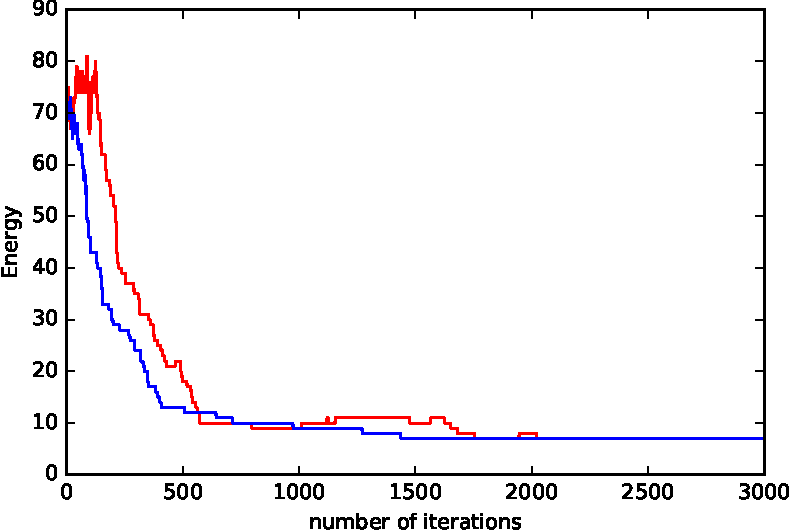
\includegraphics[width=2.3in, height = 1.7in]{H_G1_cropped.pdf}
        \caption{$G_1$}
        \label{fig:g1}
    \end{subfigure}
    ~ %add desired spacing between images, e. g. ~, \quad, \qquad, \hfill etc. 
      %(or a blank line to force the subfigure onto a new line)
    \begin{subfigure}[b]{0.45\textwidth}
        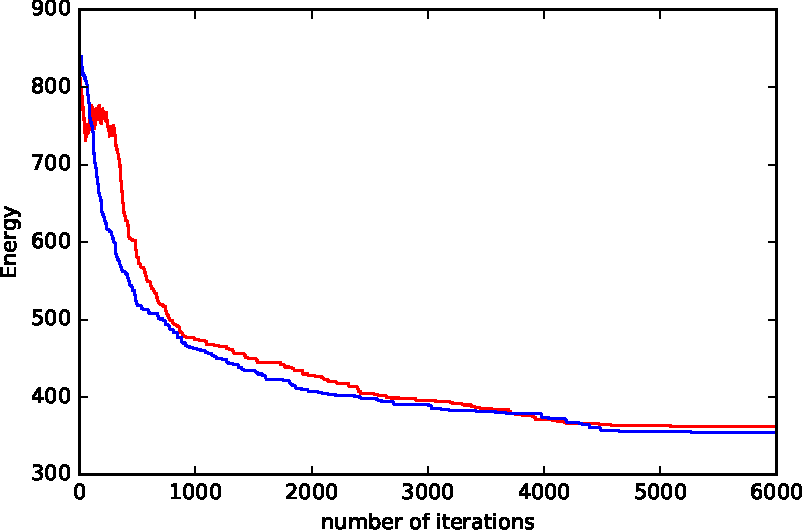
\includegraphics[width=2.3in, height=1.7in]{H_G2_cropped.pdf}
        \caption{$G_2$}
        \label{fig:g2}
    \end{subfigure}
    ~ %add desired spacing between images, e. g. ~, \quad, \qquad, \hfill etc. 
    %(or a blank line to force the subfigure onto a new line)
    \caption{Evolution of the energy of the Metropolis algorithm for two graphs. The red curve represents the evolution of the energy using a linear scheme while the blue curve represents the evolution of the energy using an exponential scheme.}
    \label{fig:comparison}
\end{figure}
\\\\
As we can see from figure \ref{fig:comparison}, results are pretty similar. The exponential schedule tends to decrease faster but obtains better results overall, as such, we chose this schedule to decrease the temperature.
\subsection{Epoch length}
We also tried several epoch lengths (decrease temperature every $x$ iterations), for this we used our previously chosen cooling function and again averaged results over all 4 graphs, we also set 10 000 iterations to make sure to reach convergence. we summarize our results in the following tabular:
\begin{center}
\begin{tabular}{| c || c | c| c| c| c|}
\hline
Epoch & 1 & 2 & 3 & 5 & 10\\
\hline
Average minimum Hamiltonian & 131.17 & 126.77 & 126.98 & 124.67 & 127.59\\
\hline
\end{tabular}
\captionof{table}{Epoch length results}
\end{center}
Even though differences are really small, an epoch length of 5 seems to be the most suited for our problem.
Surprisingly enough, we observed that waiting a certain amount of iterations at the beginning of the algorithm before decreasing the temperature was worse than decreasing straight away \todo{a verifier}

\bibliography{bibli_RW}
\bibliographystyle{plain}
\end{document}